\documentclass[12pt]{article}

% style
\setlength{\parindent}{0pt}
\usepackage[left=2.5cm,top=2cm,right=2.5cm,bottom=2cm,a4paper]{geometry}
\usepackage{fancyhdr}
\pagestyle{fancy}
\lhead{Team 4: TeamR2D2}
\rhead{Overzicht ontwerpspecificaties}
\renewcommand{\headrulewidth}{0.4pt}
\usepackage{lscape}
\usepackage{hyperref}
\usepackage{graphicx}
\usepackage{amsmath, amssymb, amsthm}

\usepackage{siunitx}
\usepackage[dutch]{babel}

\usepackage{translator}

\usepackage{longtable}
\usepackage{booktabs}
\usepackage{enumitem}
\usepackage{array}

\setlist[itemize]{noitemsep, topsep=0pt, leftmargin=*}


\begin{document}



\uselanguage{Dutch}
\languagepath{Dutch}
\providetranslation[to=Dutch]{Figure}{Figuur}



\section*{Overzicht ontwerpspecificaties}
De verkeerslichten kunnen interpreteren: stoppen bij een rood licht, doorrijden bij een groen licht:\\
De hoogte van het verkeerslicht gemeten vanaf de grond tot aan het middelpunt van het verkeerslicht is $75mm$. Het verkeerslicht heeft een knipperfrequentie van $1Hz$. Een technische tekening van het kruispunt is te zien op \ref{fig: verkeerslicht}.
\bigskip



Een geïmplementeerd traject kunnen volgen / stoplijn detecteren:\\
De ondergrond van het traject zal ofwel donker ofwel helder zijn. De kleur van de lijnen die de auto moet volgen zal afhangen van wat de kleur van de ondergrond is. Het zal het omgekeerde zijn waardoor het verschil duidelijk is. Er zijn ook nog verschillen in de soorten lijnen die op de ondergrond aangebracht zullen worden. De breedte van een volglijn is $25mm$ en de breedte van een stoplijn is $50mm$. De kruispunten liggen op $1000mm$ van elkaar en figuur \ref{fig: kruispunt} toont het bovenaanzicht van een kruispunt. 


\bigskip


Commando's van een computer kunnen volgen:\\
Vooraleer onze auto het traject mag oprijden, moeten we eerst op afstand een noodstop kunnen uitvoeren. 



\bigskip

De auto moet aan een bepaald budget voldoen:\\
Er is een budget van $3500$ eenheden beschikbaar. Dit budget kunnen we gebruiken om materiaal aan te kopen op de site: http://www.irkulak.be/po2/.
Verder kunnen we het budget ook nog gebruiken om onze eigen ontwerpen te 3D-printen. 

\bigskip
Het volledige traject foutloos kunnen afleggen met een aanvaardbaar tempo:\\
De wagen heeft een maximumbreedte van $250mm$, een maximumhoogte van $300mm$ en een minimumhoogte van $75mm$.

\bigskip

\begin{figure}
	\centering
	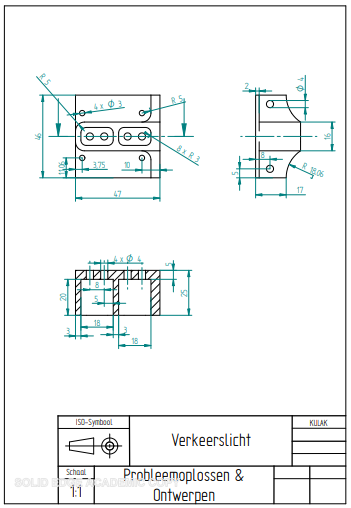
\includegraphics[width=.8\textwidth]{verkeerslicht}
	\caption{Technische tekening verkeerslicht, opgehaald van \cite{artikel1}. }
	\label{fig: verkeerslicht}
\end{figure}
\bigskip
\begin{figure}
	\centering
	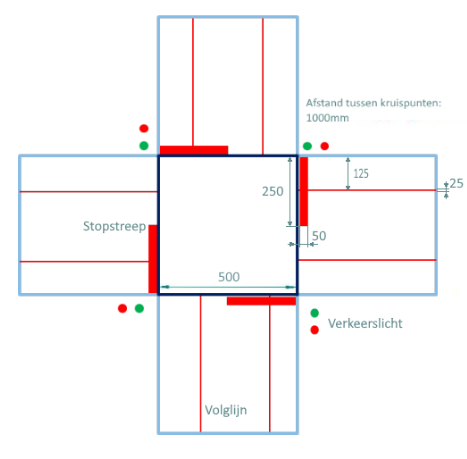
\includegraphics[width=.8\textwidth]{bovenaanzichtkruispunt}
	\caption{Bovenaanzicht kruispunt met relevante maten en items, aangepast vanuit \cite{Smart}.
	}
	\label{fig: kruispunt}
\end{figure}






\bibliography{ontwerps}
\bibliographystyle{unsrt}


\end{document}